%----------------------------------------------------------------------------------------
%	PACKAGES AND OTHER DOCUMENT CONFIGURATIONS
%----------------------------------------------------------------------------------------

\documentclass[fontsize=12pt, paper=a4, headinclude, twoside=false, parskip=half+, pagesize=auto, numbers=noenddot, open=right]{scrreprt} %{article}

\usepackage[left= 2cm,right = 2cm, bottom = 2 cm]{geometry}
\usepackage[onehalfspacing]{setspace}
\usepackage[german]{babel}
\usepackage[utf8x]{inputenc}
\usepackage{amsmath}
\usepackage{graphicx}
\usepackage{epstopdf}
\usepackage[colorinlistoftodos]{todonotes}
\graphicspath{{images/}}
\usepackage{fancyhdr}
\usepackage{caption}
\usepackage{pdfpages}
\usepackage[export]{adjustbox}
\usepackage[T1]{fontenc}            % Ermöglicht die automatische Trennung von Worten mit Umlauten
\usepackage{amssymb}
\usepackage{ltxtable}
\usepackage{booktabs-de}
\usepackage{caption}
 
% Dokumentinformationen
\usepackage[
	pdftitle={Dokumentation TaskY},
	pdfsubject={Softwaredokumentation},
	pdfauthor={Michael Müller},
	pdftex=true, 
	colorlinks=true,
 	breaklinks=true,
	citecolor=black,
	linkcolor=black,	
	menucolor=black,	
	urlcolor=black
]{hyperref}

% fussnote ganz am Ende der Seite
\usepackage[bottom]{footmisc}

%  Bibliographie
\usepackage{bibgerm} % Umlaute in BibTeX
\usepackage{csquotes}

% nicht einrücken nach Absatz
\setlength{\parindent}{0pt}

\def\code#1{\texttt{#1}}
\usepackage{etoolbox}
\makeatletter
\gdef\tshortstack{\@ifnextchar[\@tshortstack{\@tshortstack[c]}}
\let\@tshortstack\@shortstack
\patchcmd\@tshortstack\vbox\vtop{}{}
\makeatother


\begin{document}

\pagestyle{empty}
\begin{titlepage}

\newcommand{\HRule}{\rule{\linewidth}{0.5mm}} % Defines a new command for the horizontal lines, change thickness here

\center % Center everything on the page
 
%----------------------------------------------------------------------------------------
%	HEADING SECTIONS
%----------------------------------------------------------------------------------------

\LARGE Hochschule für Telekommunikation Leipzig (HfTL)\\[1.2cm] % Name of your university/college
\textsc{\Large Profilierung Netzbasierte Anwendungen}\\[0.5cm] % Major heading such as course name
\textsc{\Large Profilierung Mobile Applikationen}\\[0.5cm] % Major heading such as course name
\textsc{\large Softwaredokumentation}\\[0.5cm] % Minor heading such as course title

%----------------------------------------------------------------------------------------
%	TITLE SECTION
%----------------------------------------------------------------------------------------

\HRule \\[0.4cm]
{ \LARGE \bfseries TaskY - Cache und Notifications in mobilen Webanwendungen}\\ % Title of your document
\HRule \\[1cm]
 
%----------------------------------------------------------------------------------------
%	AUTHOR SECTION
%----------------------------------------------------------------------------------------

\Large David Howon (147102)\\[1cm] 

\Large Michael Müller (147105)\\[1cm] 

%----------------------------------------------------------------------------------------
%	DATE SECTION
%----------------------------------------------------------------------------------------

{\large Wintersemester 2016/17}\\[2cm] % Date, change the \today to a set date if you want to be precise

%----------------------------------------------------------------------------------------
%	LOGO SECTION
%----------------------------------------------------------------------------------------


\includegraphics[width=0.4\textwidth]{hftl_logo.eps}\\[1cm] % Include a department/university logo - this will require the graphicx package
 
%----------------------------------------------------------------------------------------

\vfill % Fill the rest of the page with whitespace

\end{titlepage}

% Seitenränder anpassen
\newgeometry{
    left = 3cm, right = 4.5cm, bottom = 2.5cm
}

\renewcommand*{\chapterheadstartvskip}{\vspace*{.4\baselineskip}}% Abstand 
\renewcommand*\chapterpagestyle{fancy}

% ============= Kopf- und Fußzeile =============
\pagestyle{fancy}
%
\lhead{Dokumentation TaskY}
\chead{}
\rhead{\slshape \leftmark}
%%
\lfoot{
    
\includegraphics[scale=0.6, valign=c]{hftl_logo_sm.png}
}
\cfoot{
%{\scriptsize David Howon (147102) und Michael Müller (147105)}
}
\rfoot{\textbf{\thepage}}
%%
\renewcommand{\headrulewidth}{0.4pt}
\renewcommand{\footrulewidth}{0.0pt}

% Abstand Fussnote und Fusszeile
\setlength{\footskip}{-0.5cm} 
\setlength{\skip\footins}{0.5cm} 
% Abstand zwischen Fussnoten
\setlength{\footnotesep}{0.3cm}

% \part im Inhaltsverzeichnis nicht nummerieren
\makeatletter
\let\partbackup\l@part
\renewcommand*\l@part[2]{\partbackup{#1}{}}

\newcommand*{\quelle}{%
  \footnotesize Quelle:
}


%Seitennummerierung neu beginnen, Zahlen [arabic], röm.Zahlen [roman,Roman], Buchstaben [alph,Alph]
\pagenumbering{Roman}
\newpage
\pagestyle{fancy}
%Inhaltsverzeichnis
\tableofcontents

\newpage
%Seitennummerierung neu beginnen, Zahlen [arabic], röm.Zahlen [roman,Roman], Buchstaben [alph,Alph]
\pagenumbering{arabic}
% pagestyle für gesamtes Dokument aktivieren
\pagestyle{fancy}

\addtocontents{toc}{\protect\setcounter{tocdepth}{0}} % 0 nur > \section zeigen
\addtocontents{toc}{\protect\setcounter{tocdepth}{3}} % nur bis \subsubsection (Standard 3)

\section{Einleitung: Motivation und Ziele}

Diese Dokumentation entstand im Rahmen der Profilierungen  \glqq{}Mobile Applikationen\grqq{} und \glqq{}Netzbasierte Anwendungen\grqq{} im Wintersemester 2016/17 an der Hochschule für Telekommunikation Leipzig (HfTL). \\


Projektbericht - Bestandteile

- Motivation und Ziele\\
- Grundlagen \\
- Anforderungen \\  
- Konzeption (MVC, Methodik, + Alternativen) \\
- Implementierung \\
- Zusammenfassung und Ausblick \\


... Einleitung moderne webtechnologien --> webapps statt nativen Apps ... \\
... Beschreibung der Aufgabe/des Problems ...\\

... Versuch der Lösungsfindung/Kurzbeschreibung Projekt ... \\


\newpage

\chapter{Grundlagen}

\section{Serviceworker}
\label{sec_grundladge_serviceworker}

Ein Service Worker ist eine W3C-Standard-Webtechnik bei der JavaScript-Code im Hintergrund von Web-Browsern ausgeführt wird. Mit Hilfe von Service Worker ist es möglich, essentielle Funktionalitäten wie Caching zur Offline"=Verwendbarkeit (z.B. bei Ausfall der Internetverbindung) von Web-Anwendungen, Aktualisierungen von Inhalten im Hintergrund, aber auch die von nativen Apps bekannten Push"=Benachrichtigungen(Push"=Notifications) zu ermöglichen. Dies findet alles im Hintergrund des Browsers statt und macht somit eine Installation von Software oder Software-Diensten unnötig.

Der Service Worker kann als Proxy fungieren und zum anderen vom Server gesendete Benachrichtigungen, selbst dann empfangen, wenn gerade keine Web-Page der entsprechenden Domain / Web-App geöffnet ist. 

\section{Web Push API}
\label{sec_grundlagen_web-push}
    
Bei Web Push handelt es sich um eine Erweiterung des bekannten Service-Worker-Standards. Solange der Browser geöffnet ist, können Benachrichtigungen von Webseiten empfangen werden, selbst wenn der eigentliche Tab nicht geöffnet ist. So kann man E-Mail-Tab schließen und trotzdem über eingehende Mails informiert werden. Da keine zusätzlichen Apps oder Text-Nachrichten für direkte Notifications nötig sind, ergibt sich ein großer Vorteil für Speichernutzung, Performance und Akkulaufzeit von Mobilgeräten. \\
Web Push benötigt genauso wie die Standortfreigabe oder der Kamerazugriff eine (jederzeit wiederrufbare) Berechtigung, bevor eine Webseite auf Push-Events reagieren und Notifications anzeigen kann. 

Durch eine ständige Verbindung zu einem Push Service in unserem Fall „Firebase Cloud Messaging“ , der als zentrale Schaltstelle für Nachrichten fungiert, werden Web-Push-Benachrichtigungen ermöglicht. Ursprünglich betrieb jeder Browser-Anbieter einen eigenen Push"=Service zum Schutz der Privatsphäre. Erst kürzlich wurden aber GCM (Google Cloud Messaging Push Service von Google) und Firebase (Mozilla Firefox Push Service) zu Firebase Cloud Messaging zusammengelegt. \\
Dabei erhält jede Webseite einen anderen, anonymen Web Push Identifier zur Verhinderung von seitenübergreifenden Zuordnungen. Zudem müssen die Nutzerdaten über ein Public-Key-Verfahren verschlüsselt werden. Der Service Worker meldet sich nur beim Push-Dienst an, wenn der User die notwendigen Push"=Berechtigungen erteilt hat. 
\newpage

\section{Anforderungen}

\subsection{allgemeine Beschreibung der Applikation}

Nach erfolgreicher Registrierung und Anmeldung kann der Benutzer Aufgaben anlegen, bearbeiten, anzeigen und löschen. Weiterhin gibt es eine Kontaktliste, in welcher alle Kontakte angezeigt werden, die ebenfalls für die Anwendung registriert sind und zu persönlichen Kontakten hinzugefügt wurden. Aufgaben können mit persönlichen Kontakten geteilt werden. Ebenso ist es möglich Gruppen anzulegen, dieser Kontakte hinzuzufügen und Aufgabe mit der Gruppe zu teilen. \\

Über Änderungen an Gruppen oder Aufgaben wird der Benutzer über PUSH-Benachrichtigungen informiert. Wenn einer Aufgabe ein Benachrichtigungszeitpunkt angegeben wurde, wird ebenfalls eine PUSH-Notification angezeigt sobald die Aufgabe terminiert.


\subsection{Lösung 1: Serviceworker}

\newpage
\subsection{Lösung 2: nativer Android Dienst}

Tabelle \ref{tbl_anforderungen-android} stellt eine Auflistung von Anforderungen an die Lösung mittels nativem Android Dienst dar.
\bgroup
\def\arraystretch{1.5}%  1 is the default, change whatever you need
\begin{table}[ht]
\begin{tabularx}{\textwidth}{ |l|X|  }
    \hline
    \textbf{KRITERIUM} & \textbf{BESCHREIBUNG} \\
    \hline
    1.1 Plattform: Android & …soll für die Android Plattform entwickelt werden. Als Mindestversion soll Android 5.0 (API Level 21) vorausgesetzt werden. Eine Unterstützung anderer Betriebssysteme ist nicht vorgesehen.  \\
    \hline
    1.2 Hintergrunddienst & …soll als Hintergrunddienst ohne GUI implementiert werden. \\
    \hline
    1.3 automatischer Start & ...soll automatisch nach Systemstart gestartet werden. Wird der Dienst aus irgendeinem Grund beendet, soll er automatisch neustarten. \\
    \hline
\end{tabularx}
\caption{Anforderungen an nativen Dienst}
\label{tbl_anforderungen-android}
\end{table}
\egroup

\subsection{Web Applikation}
\subsubsection{funktionale Anforderungen}

\paragraph{[WFA-1] Benutzerauthentifizierung.} Benutzer können sich für die Nutzung der Anwendung Registrieren und anschließend Anmelden. Für die Registrierung ist ein eindeutiger Benutzername mit Angabe einer E-Mail Adresse sowie ein Passwort notwendig.

\paragraph{[WFA-2] Kontaktliste.} Benutzer können sich untereinander mittels Benutzername bzw. E-Mail Adresse zur persönlichen Kontaktliste hinzufügen.

\paragraph{[WFA-3] Gruppen verwalten. } Benutzer können Gruppen anlegen und andere Benutzer hinzufügen. Ein Gruppenadministrator kann die Gruppe bearbeiten oder löschen. Benutzer können aus einer Gruppe austreten.

\paragraph{[WFA-4] Aufgaben anlegen, bearbeiten und löschen.} Ein Benutzer soll Aufgaben anlegen und anschließend Bearbeiten oder Löschen können.
Eine Aufgabe muss einen Titel besitzen. Optional können eine Beschreibung, ein Ort, Zeitraum sowie Fälligkeitsdatum hinterlegt werden.

\paragraph{[WFA-5] Aufgaben teilen.} Aufgaben können mit mehreren Benutzer geteilt werden. Ebenfalls können Aufgaben einer Gruppe zugeordnet werden. 

\paragraph{[WFA-6] Benachrichtigungen.} Benutzer, die in einer Aufgabe involviert sind, erhalten Benachrichtigungen über Änderungen an Aufgaben. Wenn für eine Aufgabe eine Fälligkeit mit Benachrichtigung hinterlegt wurde, wird der Benutzer zum entsprechenden Zeitpunkt informiert.\\
Wird ein Benutzer in eine Gruppe eingeladen bzw. wird einer Gruppe eine Aufgaben hinzugefügt bzw. bearbeitet werden alle Gruppenmitglieder entsprechend Benachrichtigt.

\newpage
\subsubsection{nicht-funktionale Anforderungen}

\paragraph{[WNFA-1] Singlepage Applikation.}

\paragraph{[WNFA-2] Offlinefähigkeit.}

\paragraph{[WNFA-3] Look and Feel einer nativen Android App.}\label{par_wnfa3}


\newpage
\subsection{Serverkomponente}

\subsubsection{funktionale Anforderungen}

\paragraph{[SFA-1] RESTful-Schnittstelle. }Der API Server unterstützt folgende Anforderungen um die Funktionalitäten einer RESTful-Schnittstelle zu erfüllen:

\begin{itemize}  
\item Bereitstellung von CRUD\footnote{\textit{CRUD: create, read, update, delete}}-Funktionalität für Entities
\item Aufruf von Ressourcen über eindeutige und einfache URLs (z.B. https://example.de/api/task/ und https://example.de/api/task/:taskId) 
\item Verwendung der standardisierten HTTP-Methoden (GET, POST, PUT und DELETE) 
\item Rückgabe im JSON-Format
\item alle Requests werden auf der Konsole ausgegeben
\end{itemize}


\paragraph{[SFA-2] Gesicherter Zugriff auf API.} Der Zugriff auf die API ist nur für authentifizierte Benutzer möglich. Für die Authentifizierung wird das Konzept Token verwendet. \\
\textbf{KONZEPT TOKEN BESCHREIBEN}


\subsubsection{nicht-funktionale Anforderungen}
ssdf



\newpage

\chapter{Konzeption}
\label{sec_konzeption}

\section{Umsetzung mittels Serviceworker}
\label{subsec_konzeption_serviceworker}

\subsection{Architekturbeschreibung}
\label{subsubsec_konzeption_serviceworker_architektur}

Die Anwendung beruht auf dem Client-Server-Prinzip. Dabei stellt der Client lediglich die Oberfläche zur Interaktion mit dem Anwender dar. Außer der notwendigen UI Logik ist die gesamte Geschäftslogik auf einen dedizierten (Business-)Server ausgelagert. Dieser stellt ebenfalls die Datenbank bereit. Mittels AJAX und REST werden dynamische Daten vom Client beim Server angefragt.

\begin{figure}[htp] \centering{
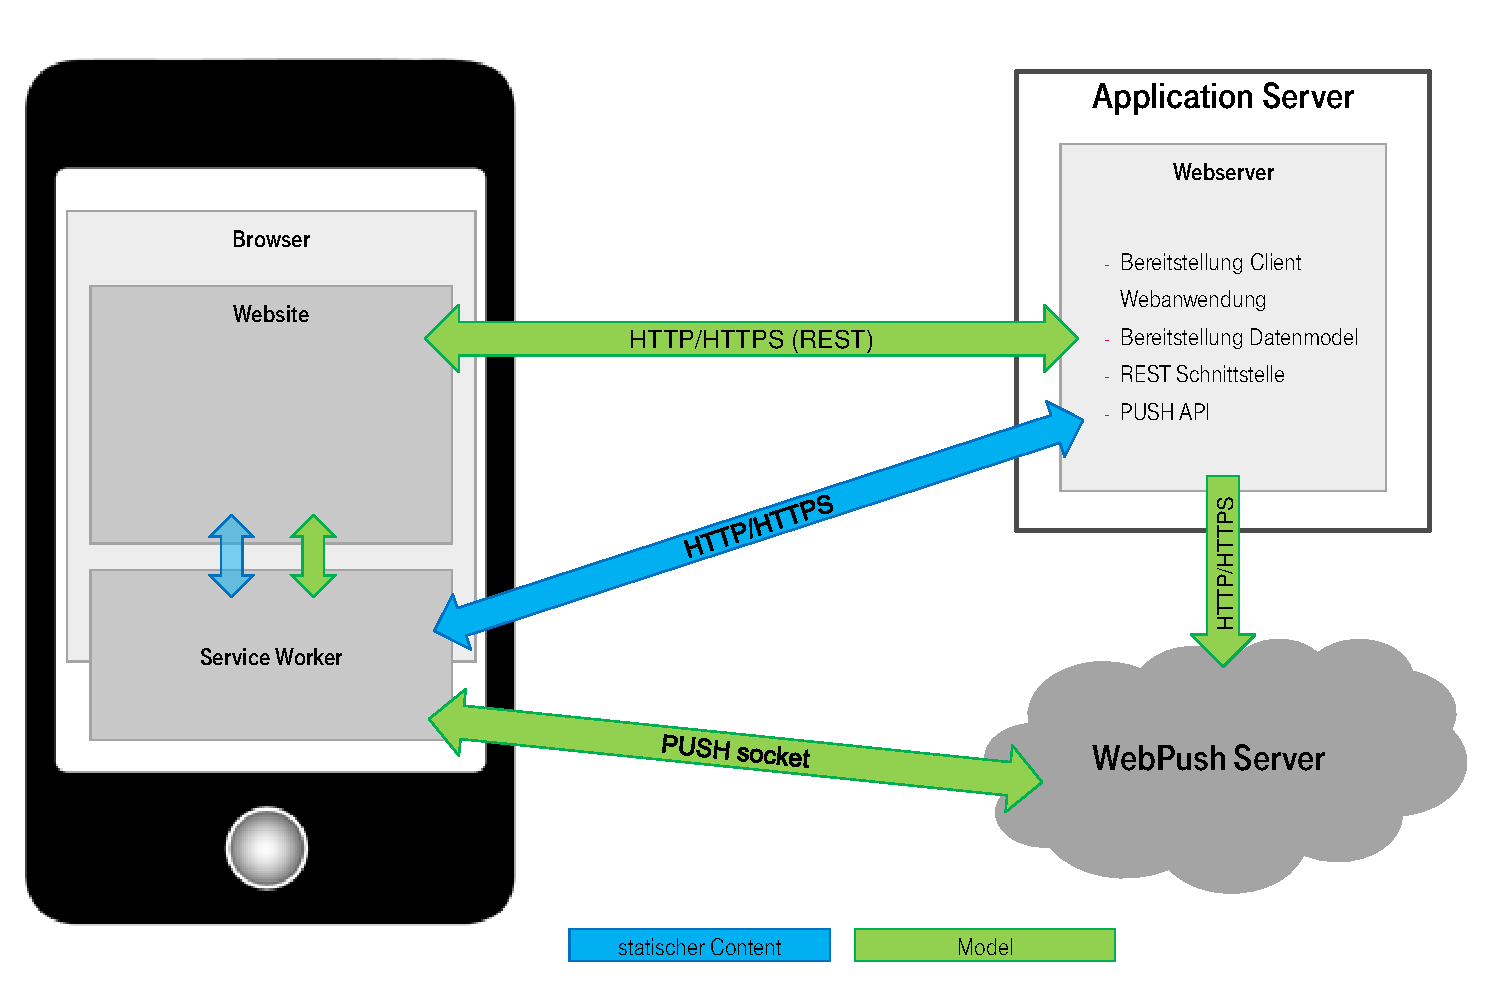
\includegraphics[width=0.9\textwidth]{images/architektur_serviceworker.pdf}}
\caption{Archtikturbeschreibung - Umsetzung mit Serviceworker}
\label{image_architektur-serviceworker-push}
\end{figure} 

\newpage
\subsection{Push API}
\label{subsubsec_konzeption_serviceworker_push-api}

\begin{figure}[htp] \centering{
\centering
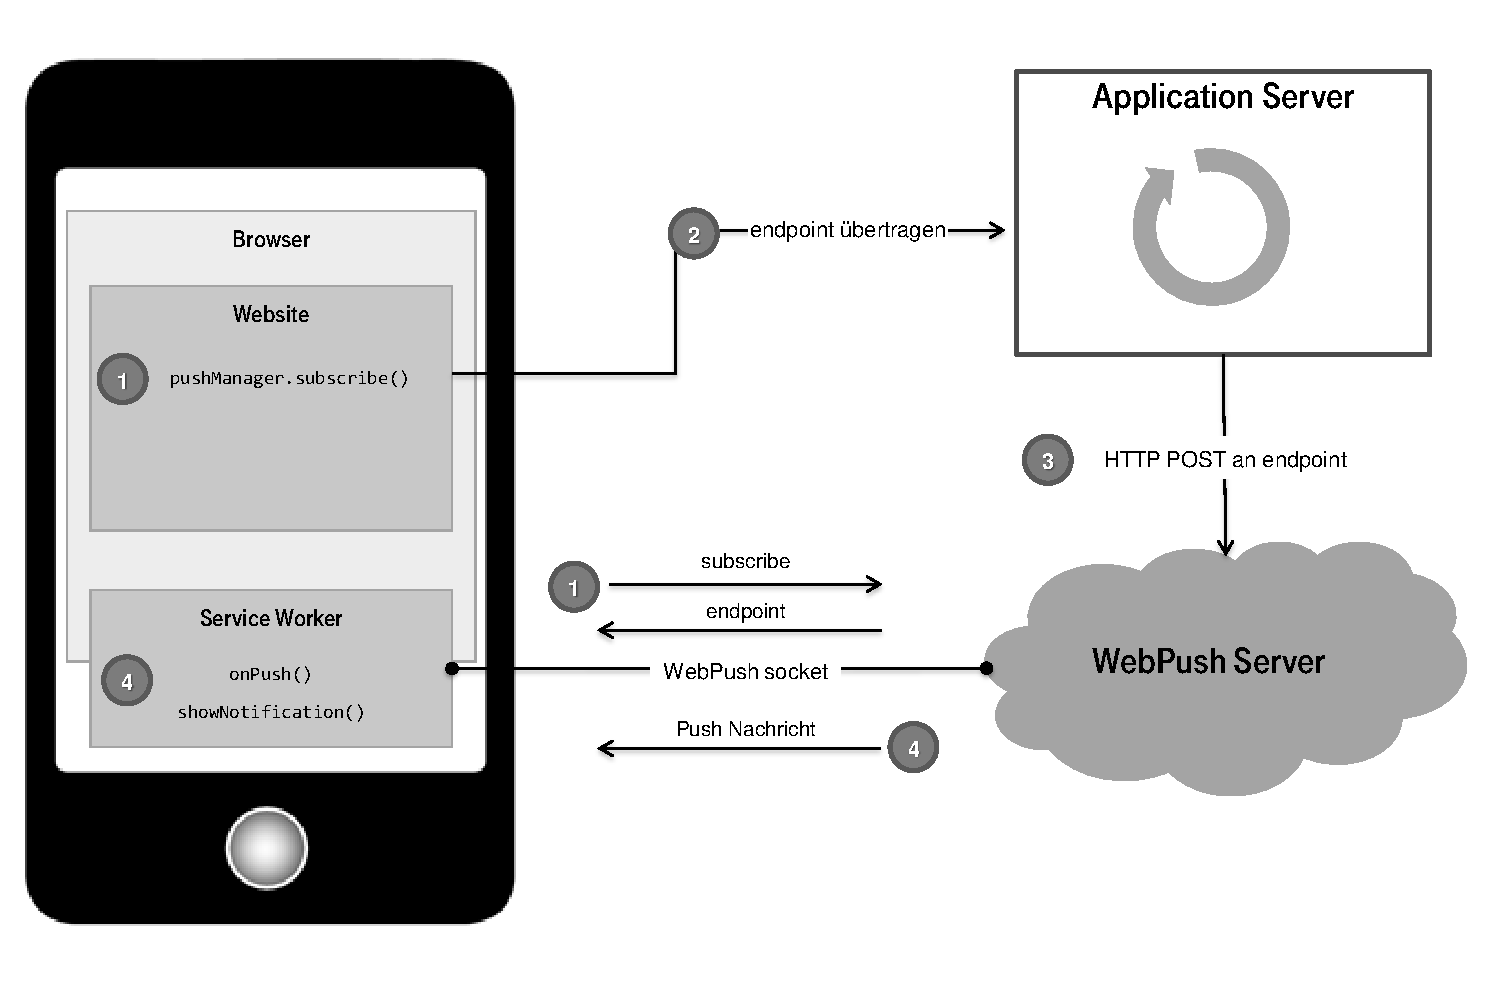
\includegraphics[width=0.9\textwidth]{images/architektur_serviceworker_push.pdf}}
\caption{Push mittels Serviceworker (in Anlehnung an MozillaWiki \cite{MOZ_WIKI})}
\quelle\url{https://wiki.mozilla.org/File:PushNotificationsHighLevel.png}
\label{image_architektur-serviceworker-push}
\end{figure}  

... Beschreibung (mit Schema) der Softwarearchitektur ...

\newpage
\section{Umsetzung mittels nativer Android Dienst}
\label{subsec_konzeption_android}

\subsection{Architekturbeschreibung}
\label{subsubsec_konzeption_android_architektur}

\begin{figure}[htp] \centering{
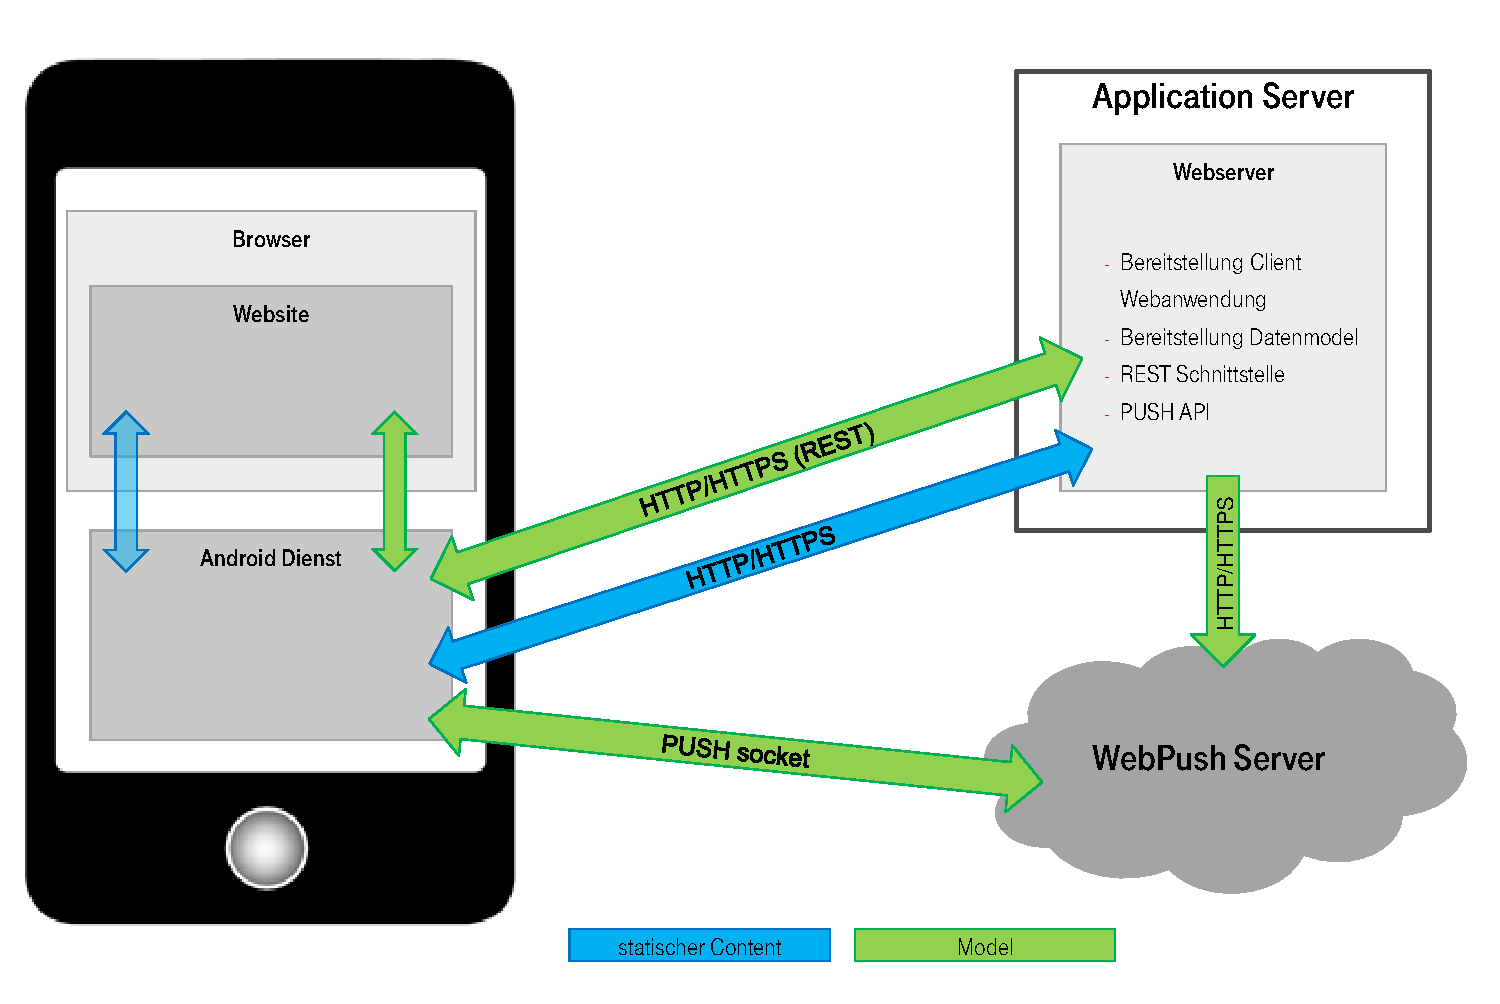
\includegraphics[width=0.9\textwidth]{images/architektur_android.pdf}}
\caption{Architektur - Umsetzung mit nativem Android Dienst }
\label{image_architektur-android-push}
\end{figure}  

... Beschreibung (mit Schema) der Softwarearchitektur ...

\newpage
\subsection{Push}

\begin{figure}[htp] \centering{
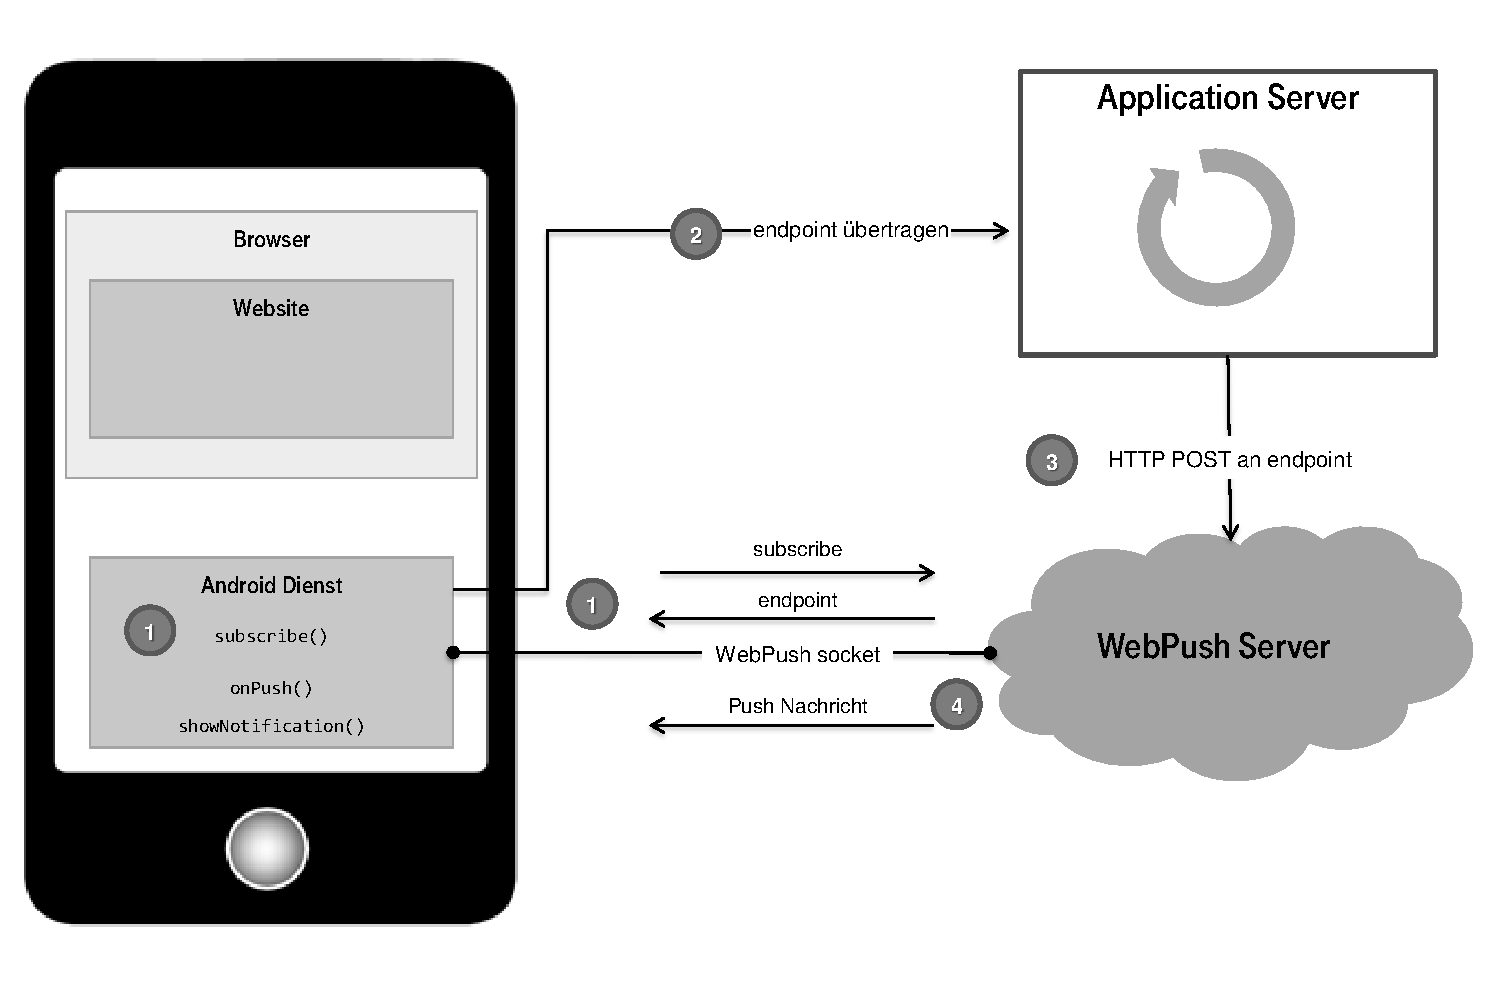
\includegraphics[width=0.9\textwidth]{images/architektur_android_push.pdf}}
\caption{Push mittels nativem Android Dienst (in Anlehnung an MozillaWiki \cite{MOZ_WIKI})}
\quelle\url{https://wiki.mozilla.org/File:PushNotificationsHighLevel.png}
\label{image_architektur-android-push}
\end{figure}  

\section{Datenmodell}
\label{subsec_datenmodell}

\begin{figure}[htp] \centering{
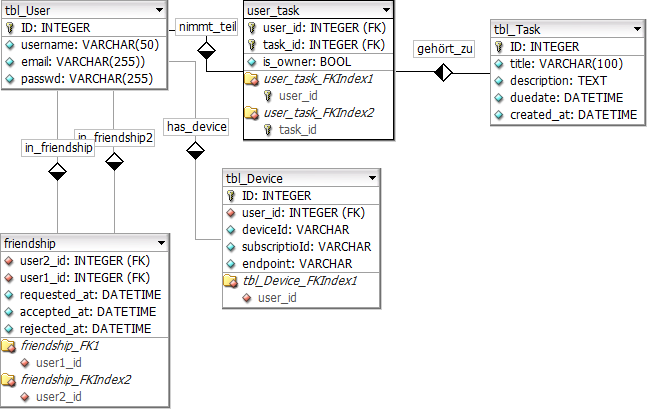
\includegraphics[width=0.9\textwidth]{images/model.png}}
\caption{Datenmodell}
\label{image_konzeption_datenmodell}
\end{figure} 


\section{Serverkomponente}
\label{subsec_serverkomponente}

\subsection{REST-API}

Zur Bereitstellung von CRUD-Funktionalitäten über standardisierte HTTP-Methoden (vgl. \ref{subsec_anforderungen_server} Anforderungen an Serverkomponente) wird dem Applicationserver eine RESTful-Schnittstelle hinzugefügt. Eine Übersicht über mögliche API-Routen mit entsprechender HTTP-Methode ist in Tabelle \ref{tbl_api-routes} dargestellt. \\

\begin{table}[h]
\centering
\begin{tabular}{l | c | l }
    \textbf{Route} & \textbf{HTTP-Methode} & \textbf{Beschreibung} \\
    \hline\hline
    /api/signup & POST & Registriert einen neuen Benutzer \\
    /api/authenticate & POST & Authentifiziert einen Benutzer \\
    \hline
    /api/tasks & GET & Gibt alle Aufgaben zurück \\
    /api/tasks & POST & Legt eine neue Aufgabe an \\
    /api/tasks/:taskId & GET & Gibt eine einzelne Aufgabe zurück \\
    /api/tasks/:taskId & PUT & Aktualisiert eine einzelne Aufgabe \\
    /api/tasks/:taskId & DELETE & Löscht eine einzelne Aufgabe \\
\end{tabular}
\caption{Übersicht API Routen}
\label{tbl_api-routes}
\end{table}

\subsubsection{Authentifizierung und Autorisierung} 

Für den Zugriff auf die CRUD-Methoden ist eine Benutzerauthentifizierung und Autorisierung notwendig. Dazu wird das Token-Verfahren verwendet.


\section{Benutzeroberfläche}

... Mockup ... \\
... Beschreibung des UI ...\\

Um das \glqq{}Look and Feel\grqq{} einer nativen App zu erreichen wird das UI-Framework \textbf{nativeDroid2} verwendet. \\

\newpage

\chapter{Implementierung}

... Wie wurden die beiden Ideen umgesetzt ...

\section{Serverkomponente}

\section{Umsetzung ServiceWorker}

... Umsetzung mittels ServiceWorker ...

\section{Umsetzung mittels nativem Android Service}

... Umsetzung mittels eigenem nativen Service ...

\begin{lstlisting}
// Hello.java
import javax.swing.JApplet;
import java.awt.Graphics;

public class Hello extends JApplet {
    public void paintComponent(Graphics g) {
        g.drawString("Hello, world!", 65, 95);
    }    
}
\end{lstlisting}

\newpage 

\section{Zusammenfassung und Ausblick}

... Was kann nicht geleistet werden? ...

... Was ist eventuell zukünftig möglich ? ...

%Literaturverzeichnis
\newpage
\bibliographystyle{unsrtdin}
%\bibliographystyle{gerplain}
\bibliography{Literatur}
\thispagestyle{fancy}

\newpage
% Abbildungsverzeichnis
\listoffigures


% ANHANG
\newpage
\addtocontents{toc}{\protect\value{tocdepth}=-1}%
\captionsetup{list=false} 
%Seitennummerierung neu beginnen, Zahlen [arabic], röm.Zahlen [roman,Roman], Buchstaben [alph,Alph]
\pagenumbering{Roman}

\section{API Beschreibung}

\begin{table}[h]
    \begin{tabular}{ l }
        Löscht eine einzelne Aufgabe \\
    \end{tabular}
    \caption{Übersicht API Routen}
    \label{tbl_api-routes}
\end{table}



{\Large \textbf{/api/signup}}


\fbox{\parbox{0.5\linewidth}{
    \textbf{Request:}
    \begin{itemize}  
        \item {\tshortstack[l]{\textbf{\code{username}}: (String)\\gewünschter Benutzername}}
        \item {\tshortstack[l]{\textbf{\code{password}}: (String)\\Passwort}}
        \item {\tshortstack[l]{\textbf{\code{email}}: (String)\\E-Mail Adresse}}
    \end{itemize}    
}
\parbox{0.5\linewidth}{
    \textbf{Response:}
    \begin{itemize}  
        \item {\tshortstack[l]{\textbf{\code{username}}: (String)\\gewünschter Benutzername}}
        \item {\tshortstack[l]{\textbf{\code{password}}: (String)\\Passwort}}
        \item {\tshortstack[l]{\textbf{\code{email}}: (String)\\E-Mail Adresse}}
    \end{itemize}    
}}

\bgroup
\def\arraystretch{1}%  1 is the default, change whatever you need

\begin{tabularx}{\textwidth}{|l|X|}
    \hline
    \multicolumn{2}{|c|}{Benutzer anlegen } \\
    \hline
    URL & \textbf{\code{/api/signup}} \\
    \hline
    Methode & \code{GET} \\
    \hline
    Request-Parameter & Required: 
      \begin{itemize}  
        \item {\tshortstack[l]{\textbf{\code{username}}: (String)\\gewünschter Benutzername}}
        \item {\tshortstack[l]{\textbf{\code{password}}: (String)\\Passwort}}
        \item {\tshortstack[l]{\textbf{\code{email}}: (String)\\E-Mail Adresse}}
      \end{itemize} \\
    \hline
    Success-Response & 
      \begin{itemize}  
        \item {Code: 200}
        \item {Content: \code{{success: true, message: 'Successful created new user.'}}}
      \end{itemize} \\
    \hline
    \multicolumn{2}{|l|}{Legt einen neuen Benutzer an. } \\
    \hline
    \multicolumn{2}{|l|}{Request } \\
    \multicolumn{2}{|l|}{ \textbf{\code{username}}: (String) gewünschter Benutzername} \\
    \multicolumn{2}{|l|}{ \textbf{\code{password}}: (String) Passwort} \\
    \multicolumn{2}{|l|}{ \textbf{\code{email}}: (String) E-Mail Adresse} \\
    \hline
\end{tabularx}
\egroup
        
\begin{itemize}  
        \item {\tshortstack[l]{\textbf{\code{username}}: (String)\\gewünschter Benutzername}}
        \item {\tshortstack[l]{\textbf{\code{password}}: (String)\\Passwort}}
        \item {\tshortstack[l]{\textbf{\code{email}}: (String)\\E-Mail Adresse}}
    \end{itemize}  
    \textbf{Response} 
    \begin{itemize}  
        \item Bereitstellung von CRUD\footnote{\textit{CRUD: create, read, update, delete}}-Funktionalität für Entities
        \item Aufruf von Ressourcen über eindeutige und einfache URLs (z.B. https://example.de/api/task/ und https://example.de/api/task/:taskId) 
    \end{itemize} 
\end{document}